\documentclass[11pt,a4paper]{article}
\usepackage[utf8]{inputenc}
\usepackage[T1]{fontenc}
\usepackage{lmodern}
\usepackage[margin=2.5cm]{geometry}
\usepackage{graphicx}
\usepackage{hyperref}
\usepackage{longtable}
\usepackage{array}
\usepackage{float}
\hypersetup{colorlinks=true,linkcolor=black,urlcolor=blue}
\setlength{\parskip}{0.5em}
\setlength{\parindent}{0pt}
\setlength{\emergencystretch}{2em}

\title{Implementação de um Serviço SOAP de Calculadora\\[0.4em]\large Desenvolvimento de Aplicações Web 2026/27 -- 1.º Trabalho Prático}
\author{Marcelo Santos\\\texttt{a79433@ualg.pt}}
\date{Outubro de 2026}

\begin{document}
\maketitle
\tableofcontents
\newpage

\section{Objetivo e âmbito}
Este relatório documenta a implementação e o consumo de um serviço SOAP sobre HTTP para as quatro operações aritméticas básicas. O serviço usa a biblioteca \texttt{soap} e as APIs HTTP de Node.js, com execução através de Bun. Os clientes disponíveis são uma aplicação web e um projeto SoapUI.

\section{Enquadramento e requisitos}
O enunciado solicita um servidor SOAP com adição, subtração, multiplicação e divisão, um WSDL que identifique entradas e saídas, validação numérica e tratamento da divisão por zero. Exige ainda um cliente capaz de visualizar requisições e respostas HTTP/SOAP, testes e documentação de execução. Os critérios de avaliação distribuem 100 pontos entre operações (20), estrutura (10), WSDL (20), validação (10), clientes (20), documentação (10) e boas práticas (10).

A solução implementada cobre as quatro operações e oferece duas formas de as consumir: uma aplicação React no navegador e o SoapUI com quatro requisições configuradas. Os testes automatizados verificam o serviço e a aplicação. Há, porém, uma diferença face à exigência literal de um cliente simples em Node.js: não existe um programa CLI Node.js separado. A demonstração programática existente é o cliente TypeScript no navegador, e os testes são executados com Bun. Esta distinção é relevante na avaliação.

\section{Tecnologias e organização}
O serviço está em TypeScript e usa \texttt{node:http} para criar o servidor HTTP, \texttt{node:fs} para ler o contrato e a biblioteca npm \texttt{soap} (versão 1.14.0) para publicar as operações. O ambiente de execução usado é Bun 1.4.4, compatível com as APIs de Node.js utilizadas; portanto, não se afirma que o processo esteja a correr no binário \texttt{node}. A interface usa React e \texttt{fetch} para criar e enviar XML SOAP 1.1 diretamente a partir do navegador.

\begin{center}
\small
\begin{tabular}{|p{3.4cm}|p{10cm}|}
\hline
\textbf{Elemento} & \textbf{Responsabilidade} \\ \hline
\path{soap-server/src/index.ts} & Implementação das operações, verificação de operandos e resultados, publicação SOAP e política CORS. \\ \hline
\path{soap-server/src/service.wsdl} & Contrato de mensagens, operações, binding SOAP e endereço do serviço. \\ \hline
\path{soap-app/src/service.ts} & Criação do envelope, envio HTTP, interpretação da resposta e dos faults. \\ \hline
\path{soap-app/src/APITester.tsx} & Formulário e visualização de resultado, detalhes HTTP e XML das duas direções. \\ \hline
\texttt{compose.yaml} e \texttt{Dockerfile} & Três serviços: backend, frontend e desktop remoto do SoapUI. \\ \hline
\end{tabular}
\end{center}

O fluxo de uma operação é: o utilizador escolhe a operação e os números; o cliente constrói um \texttt{Envelope} XML; envia um \texttt{POST} com \texttt{Content-Type: text/xml} e \texttt{SOAPAction}; a biblioteca \texttt{soap} encaminha a operação publicada no WSDL; a lógica valida, calcula e devolve \texttt{result}, ou gera um \texttt{SOAP Fault}. O cliente interpreta o \texttt{Body} pelo namespace SOAP e apresenta o XML e o estado HTTP.

\section{Contrato WSDL e operações}
O contrato é publicado em \url{http://localhost:3000/wsdl?wsdl}; as chamadas SOAP são dirigidas a \url{http://localhost:3000/wsdl}. O \texttt{targetNamespace} é \url{http://example.org}. O WSDL define mensagens de pedido com duas partes, \texttt{a} e \texttt{b}, e mensagens de resposta com uma parte \texttt{result}; todas são declaradas \texttt{xsd:double}. O \texttt{portType} contém quatro operações de pedido/resposta. O binding usa SOAP sobre HTTP, estilo \texttt{rpc} e \texttt{literal}, com \texttt{soapAction} igual ao nome da operação.

\begin{center}
\begin{tabular}{|l|l|l|l|}
\hline
\textbf{Operação} & \textbf{Argumentos} & \textbf{Cálculo} & \textbf{Exemplo} \\ \hline
\texttt{Add} & \texttt{a, b} & $a+b$ & $2+3=5$ \\ \hline
\texttt{Subtract} & \texttt{a, b} & $a-b$ & $9-4=5$ \\ \hline
\texttt{Multiply} & \texttt{a, b} & $a\times b$ & $6\times7=42$ \\ \hline
\texttt{Divide} & \texttt{a, b} & $a/b$ & $8/2=4$ \\ \hline
\end{tabular}
\end{center}

Por exemplo, a operação \texttt{Add} dispõe das mensagens \texttt{AddRequest} e \texttt{AddResponse}; o mesmo padrão é repetido para as restantes operações. O WSDL é lido no arranque, e o endereço publicado é atualizado de acordo com \verb|SOAP_PORT|. A tipagem \texttt{xsd:double} descreve o contrato numérico; a validação adicional de valores finitos é feita na implementação do serviço.

\section{Implementação do servidor e validação}
A função \texttt{calculate} centraliza a verificação de entrada e saída, evitando regras diferentes nas quatro operações. Primeiro recusa operandos inexistentes, nulos ou constituídos apenas por espaços. Depois converte os valores com \texttt{Number} e rejeita aqueles que não são finitos, como \texttt{NaN} e \texttt{Infinity}. Por fim, verifica que o resultado também é finito. A divisão adiciona uma regra explícita: quando \texttt{b=0}, gera \texttt{faultstring} igual a \texttt{divisao por zero}.

Os erros de entrada são expostos como \texttt{SOAP Fault} com \texttt{faultcode} \texttt{Client} e estado HTTP 500. Por exemplo, \texttt{Add(oops, 2)} é rejeitado como entrada não numérica, e \texttt{Divide(1, 0)} não devolve \texttt{Infinity}. Em vez disso, a resposta contém uma falha SOAP legível pelo cliente. Uma política CORS autoriza a origem da interface web e responde a preflight \texttt{OPTIONS}, necessário porque o navegador envia \texttt{SOAPAction} e XML por \texttt{POST}.

\section{Exemplos do protocolo}
O exemplo seguinte representa uma chamada SOAP 1.1 para \texttt{Add(2,3)}. O servidor recebe um pedido HTTP \texttt{POST /wsdl} com \texttt{Content-Type: text/xml; charset=utf-8} e \texttt{SOAPAction: Add}. Prefixos de namespace como \texttt{tns} e \texttt{exam} são equivalentes quando indicam o mesmo URI.

{\small\begin{verbatim}
<soap:Envelope xmlns:soap="http://schemas.xmlsoap.org/soap/envelope/"
							 xmlns:tns="http://example.org">
	<soap:Body>
		<tns:Add><a>2</a><b>3</b></tns:Add>
	</soap:Body>
</soap:Envelope>
\end{verbatim}}

Uma resposta bem-sucedida tem HTTP 200 e a parte \texttt{result} dentro de \texttt{AddResponse}:

{\small\begin{verbatim}
<soap:Envelope xmlns:soap="http://schemas.xmlsoap.org/soap/envelope/"
							 xmlns:tns="http://example.org">
	<soap:Body>
		<tns:AddResponse><tns:result>5</tns:result></tns:AddResponse>
	</soap:Body>
</soap:Envelope>
\end{verbatim}}

Para \texttt{Divide(1,0)}, a resposta real apresenta HTTP 500 e o seguinte conteúdo lógico dentro de \texttt{soap:Body}:

{\small\begin{verbatim}
<soap:Fault>
	<faultcode>Client</faultcode>
	<faultstring>divisao por zero</faultstring>
</soap:Fault>
\end{verbatim}}

As capturas da Figura~\ref{fig:web-soma} e da Figura~\ref{fig:web-fault} mostram os estados HTTP e os documentos SOAP expostos lado a lado pelo cliente web. Os cabeçalhos apresentados pela interface são os disponibilizados ao JavaScript do navegador; a inspeção integral do transporte pode ser feita nas ferramentas de rede do navegador ou no SoapUI.

\begin{figure}[p]
\centering
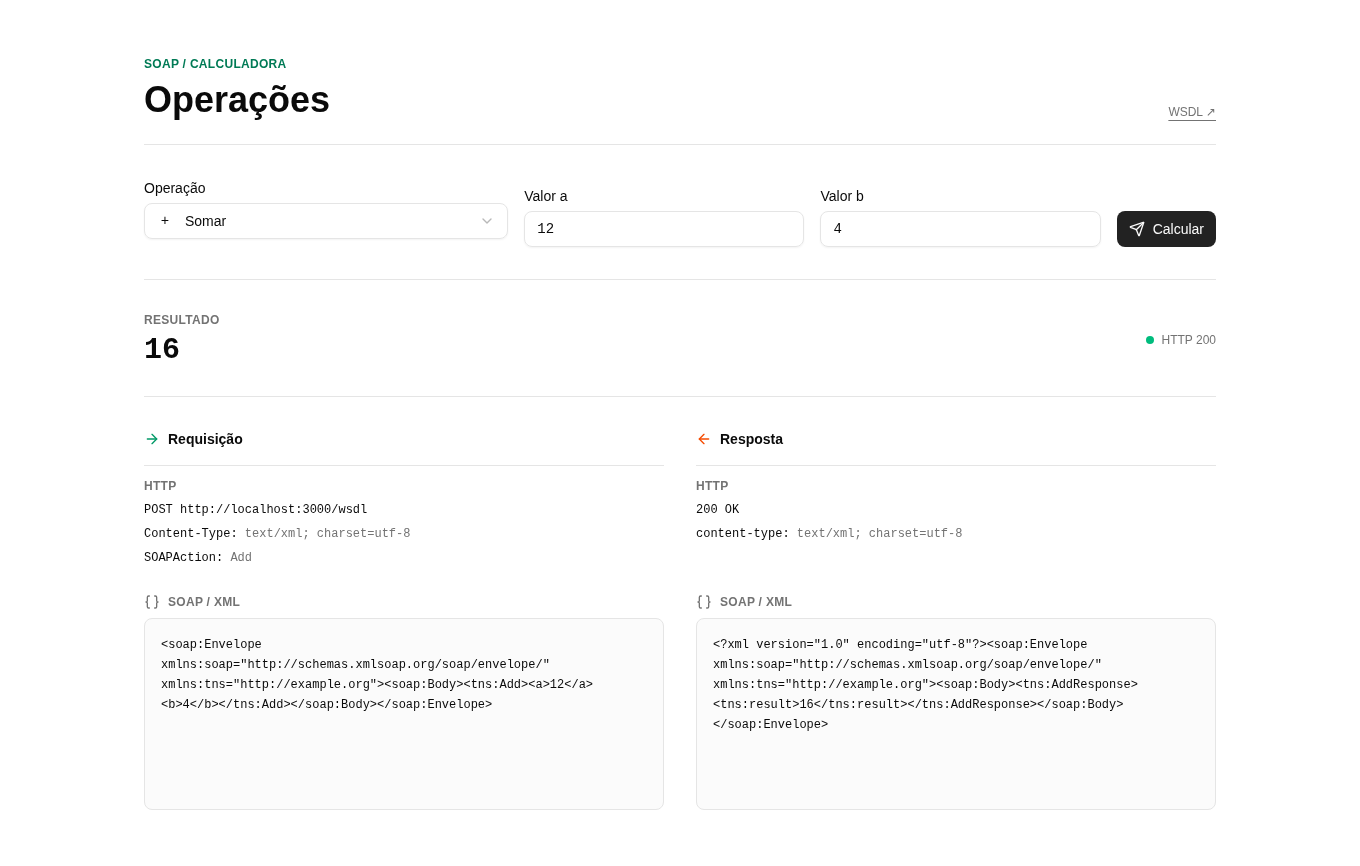
\includegraphics[width=\linewidth,height=0.73\textheight,keepaspectratio]{figuras/cliente-web-soma.png}
\caption{Cliente web: requisição Add(12,4), estado HTTP 200 e resultado 16 no XML da resposta.}
\label{fig:web-soma}
\end{figure}

\begin{figure}[p]
\centering
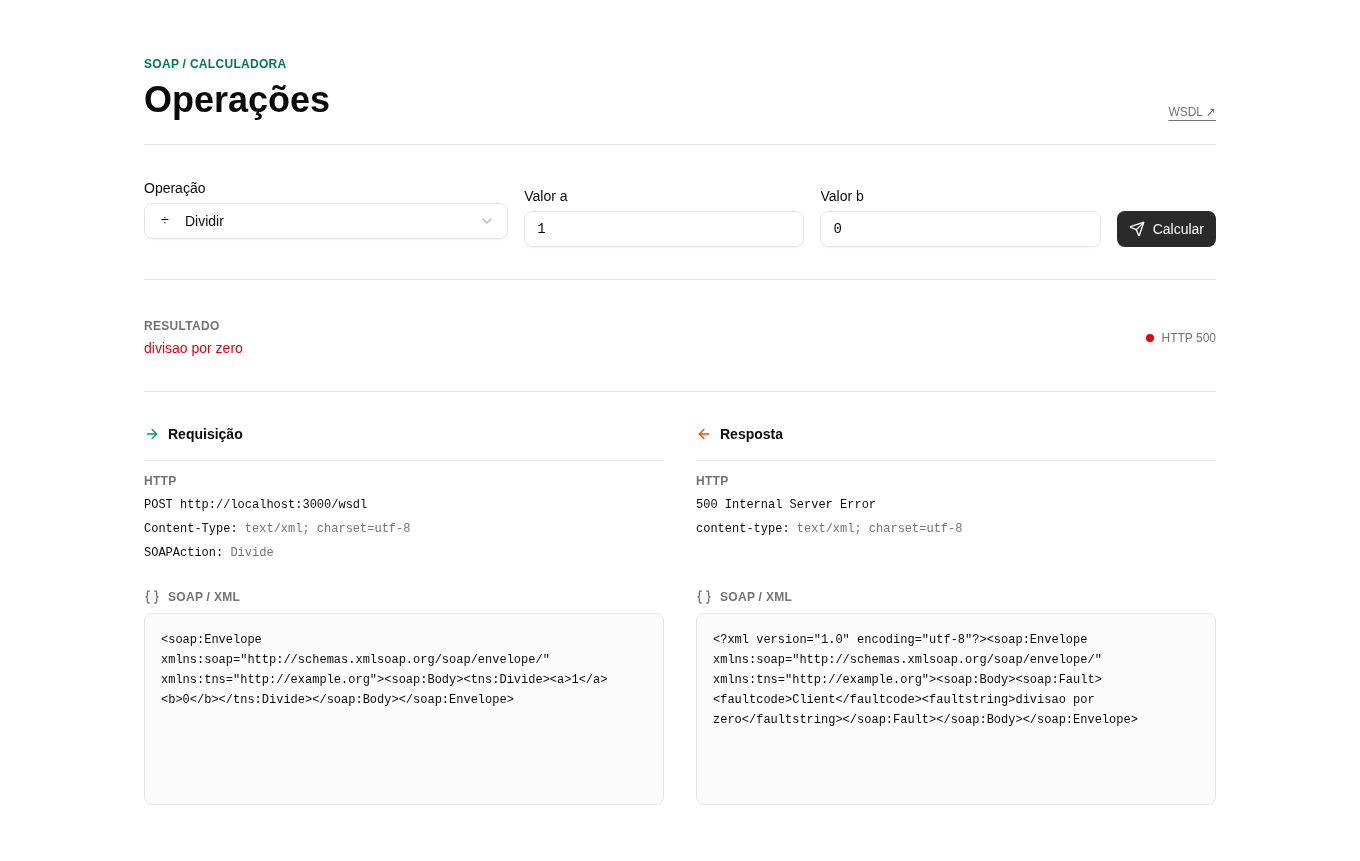
\includegraphics[width=\linewidth,height=0.73\textheight,keepaspectratio]{figuras/cliente-web-fault.png}
\caption{Cliente web: Divide(1,0), estado HTTP 500 e SOAP Fault com a mensagem de divisão por zero.}
\label{fig:web-fault}
\end{figure}

\clearpage
\section{Clientes e demonstração no SoapUI}
No cliente web, o formulário recebe a operação e dois números. Antes da chamada, recusa entradas vazias e não finitas; \texttt{service.ts} obtém a URL de \texttt{/api/config}, monta o envelope SOAP e envia-o por \texttt{fetch}. O XML da resposta é analisado com \texttt{DOMParser}; o cliente procura um \texttt{Fault} no \texttt{Body} ou um elemento \texttt{OperationResponse} com \texttt{result}. São conservados o pedido, a resposta, o resultado e eventuais mensagens de erro, para que o ecrã mostre o tráfego e não apenas o número calculado.

O SoapUI 5.9.1 está acessível como aplicação gráfica num desktop XFCE remoto em \url{https://localhost:8080/} (certificado local autoassinado). O projeto \texttt{Calculadora SOAP} foi importado a partir de \url{http://soap-server:3000/wsdl?wsdl} e guardado no volume persistente \texttt{soapui-config}, no ficheiro \texttt{/config/Calculadora-SOAP-soapui-project.xml}. Contém uma requisição de exemplo por operação, com valores válidos e endpoint \url{http://soap-server:3000/wsdl}.

Esta diferença de endereços é deliberada: \texttt{localhost:3000} é apropriado para o navegador no host; no contêiner do SoapUI, \texttt{localhost} apontaria para o próprio desktop remoto. Por isso, o SoapUI usa o nome de serviço \texttt{soap-server} da rede Docker Compose. O WSDL anuncia \texttt{localhost} para o consumidor no host; a definição importada no SoapUI e as respetivas requisições usam a URL interna. O projeto guardado mantém estas escolhas entre reinícios, desde que o volume não seja removido.

\begin{figure}[p]
\centering
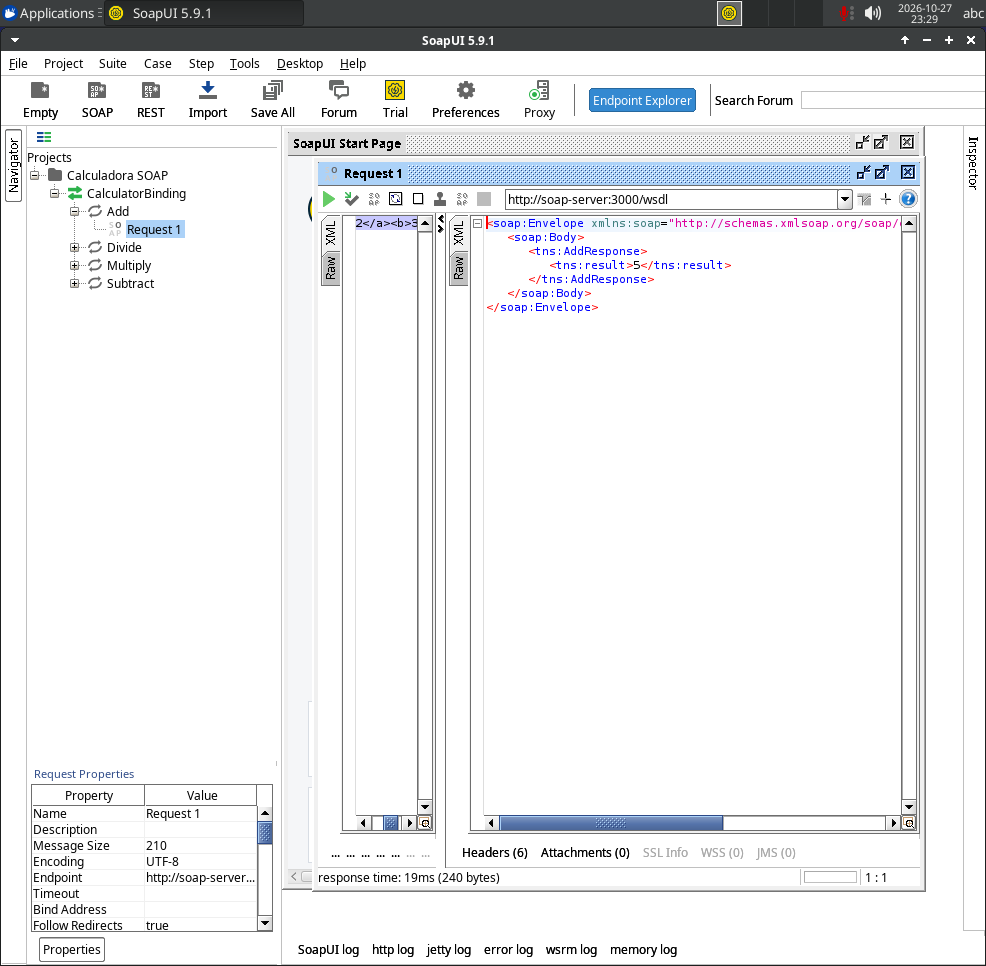
\includegraphics[width=\linewidth,height=0.67\textheight,keepaspectratio]{figuras/soapui-soma.png}
\caption{SoapUI com a operação Add(2,3): resposta SOAP recebida com resultado 5.}
\label{fig:soapui-add}
\end{figure}

\begin{figure}[p]
\centering
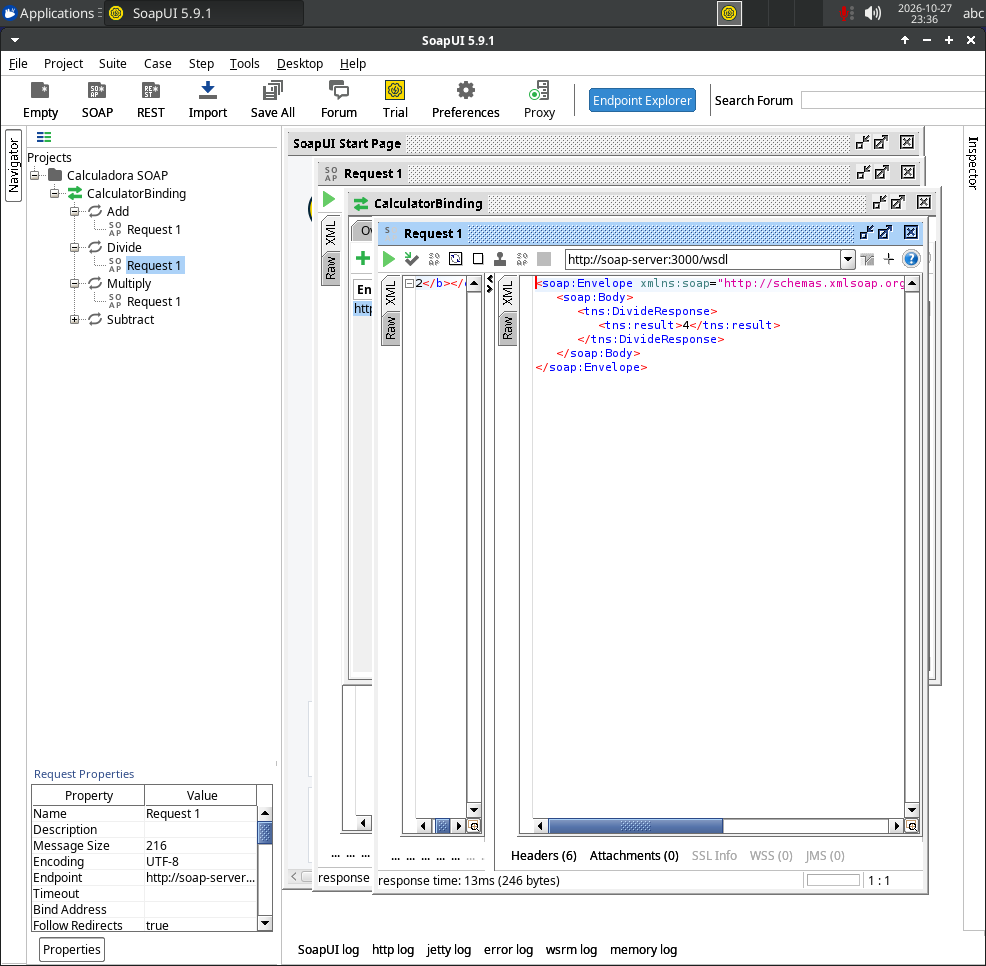
\includegraphics[width=\linewidth,height=0.67\textheight,keepaspectratio]{figuras/soapui-divisao.png}
\caption{SoapUI com a operação Divide(8,2): resposta SOAP com resultado 4.}
\label{fig:soapui-div}
\end{figure}

\begin{figure}[p]
\centering
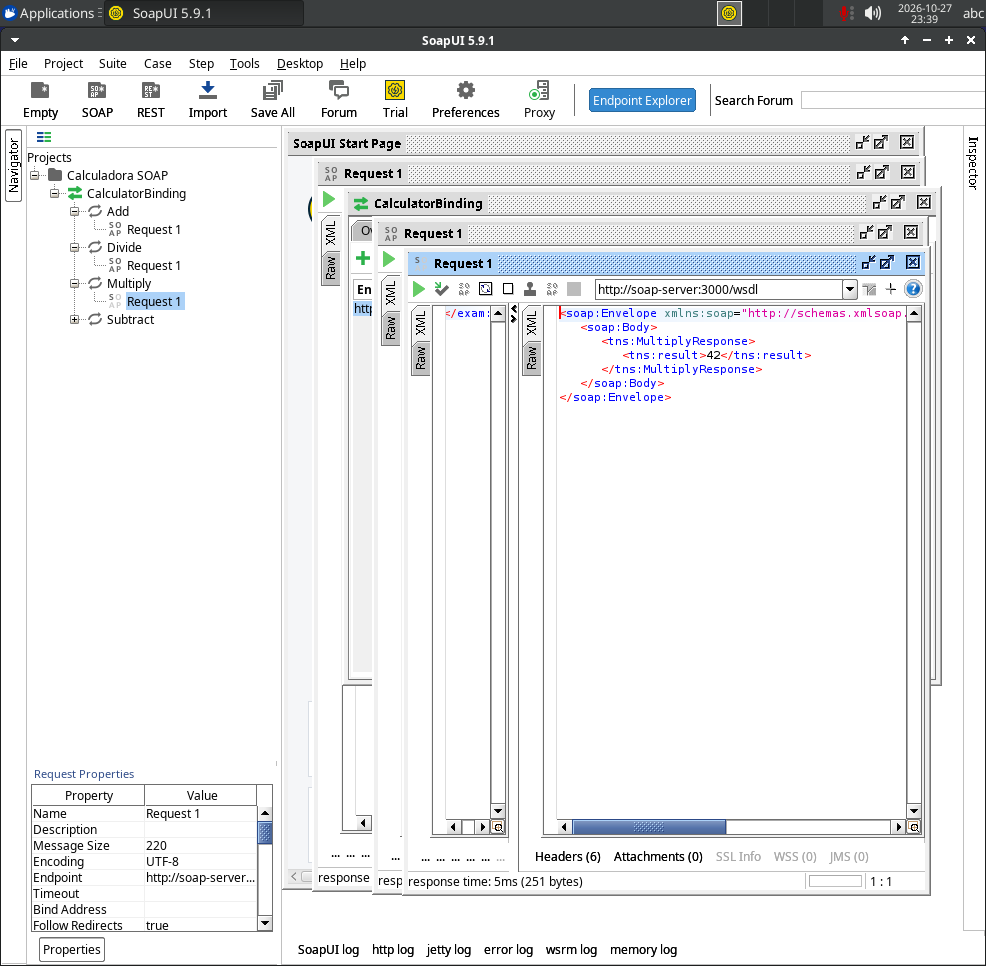
\includegraphics[width=\linewidth,height=0.67\textheight,keepaspectratio]{figuras/soapui-multiplicacao.png}
\caption{SoapUI com a operação Multiply(6,7): resposta SOAP com resultado 42.}
\label{fig:soapui-mul}
\end{figure}

\begin{figure}[p]
\centering
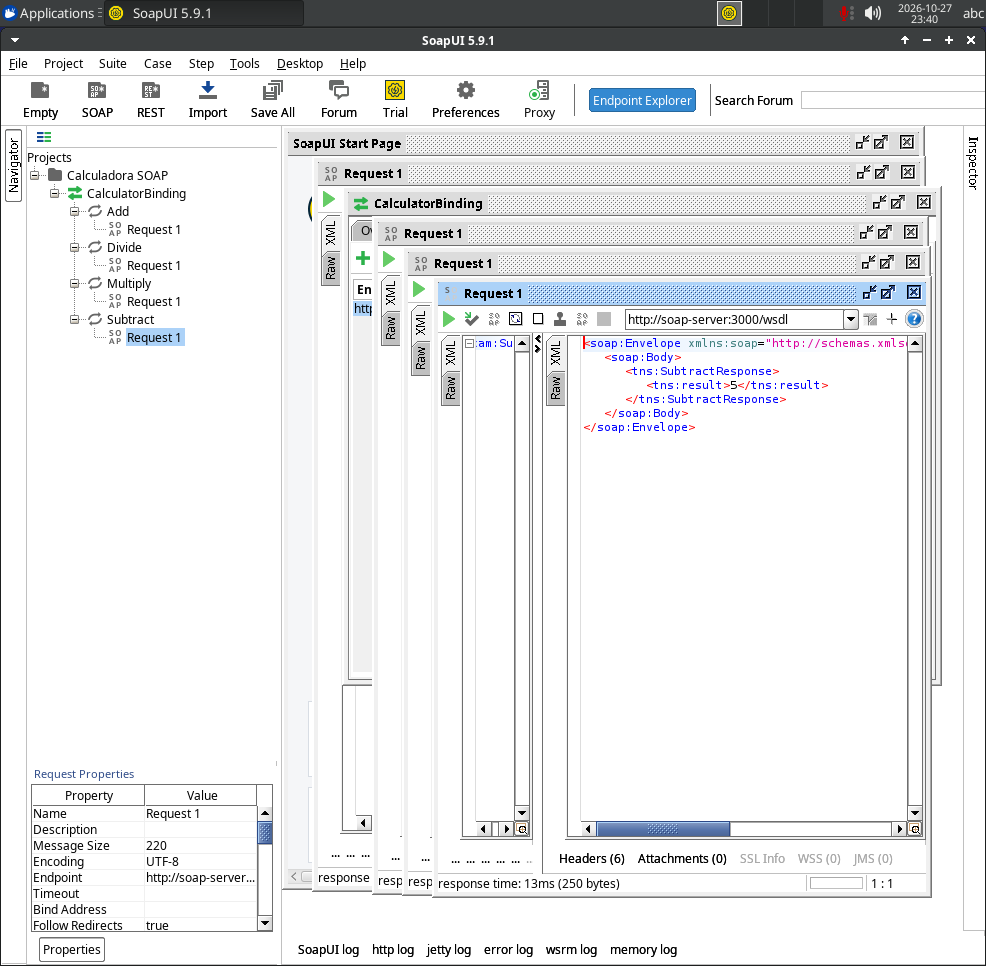
\includegraphics[width=\linewidth,height=0.67\textheight,keepaspectratio]{figuras/soapui-subtracao.png}
\caption{SoapUI com a operação Subtract(9,4): resposta SOAP com resultado 5.}
\label{fig:soapui-sub}
\end{figure}

\clearpage
\section{Testes e resultados observados}
Foram executadas as suites \texttt{bun test} de ambos os pacotes: \textbf{12 testes passaram no servidor} e \textbf{6 testes passaram na aplicação}, sem falhas. Os testes do servidor verificam a publicação do WSDL, as quatro operações, entradas inválidas (incluindo valores vazios, \texttt{NaN} e \texttt{Infinity}), operandos ausentes, divisão por zero e CORS. Os testes do cliente usam Chromium para verificar as respostas e os detalhes HTTP/XML, faults, XML malformado, indisponibilidade do serviço, validação local e ausência de deslocamento horizontal no ecrã móvel.

\begin{center}
\small
\begin{tabular}{|p{3.1cm}|p{2.3cm}|p{2.7cm}|p{5.2cm}|}
\hline
\textbf{Cenário} & \textbf{Entrada} & \textbf{HTTP / saída} & \textbf{Evidência} \\ \hline
Soma & 2, 3 & 200 / 5 & SoapUI, Figura~\ref{fig:soapui-add} \\ \hline
Subtração & 9, 4 & 200 / 5 & SoapUI, Figura~\ref{fig:soapui-sub} \\ \hline
Multiplicação & 6, 7 & 200 / 42 & SoapUI, Figura~\ref{fig:soapui-mul} \\ \hline
Divisão & 8, 2 & 200 / 4 & SoapUI, Figura~\ref{fig:soapui-div} \\ \hline
Divisão por zero & 1, 0 & 500 / SOAP Fault & Cliente web, Figura~\ref{fig:web-fault}; testes \\ \hline
Argumento inválido & \texttt{oops}, 2 & 500 / SOAP Fault & Teste automatizado do servidor \\ \hline
\end{tabular}
\end{center}

As quatro requisições de exemplo do projeto SoapUI foram inspecionadas após guardar: as quatro usam o endpoint interno e contêm os operandos indicados na tabela. As capturas são evidência visual das chamadas manuais; os resultados das suites referem-se à execução automatizada descrita acima e não substituem a inspeção do protocolo.

\section{Instalação, execução e entrega}
Sem Docker, é necessário instalar Bun. Na pasta \texttt{soap-server}, executar \texttt{bun install} e \texttt{bun src/index.ts}; noutra consola, na pasta \texttt{soap-app}, executar \texttt{bun install} e \texttt{bun dev}. Abrir \url{http://localhost:3001/} e consultar o contrato em \url{http://localhost:3000/wsdl?wsdl}. Para executar os testes, usar \texttt{bun test} em cada pasta.

Com Docker Compose, executar \texttt{docker compose up --build} na raiz do repositório. O backend fica na porta 3000, a aplicação na 3001 e o SoapUI em \url{https://localhost:8080/}. A porta do SoapUI está limitada a \texttt{127.0.0.1}. Aceitar o certificado autoassinado ao abrir o desktop; selecionar uma das quatro requisições existentes no projeto \texttt{Calculadora SOAP} e premir o botão de envio. Não usar \texttt{docker compose down -v} se se pretender conservar o projeto no volume.

O código do serviço está em \path{soap-server/}, o cliente em \path{soap-app/}, o WSDL em \path{soap-server/src/service.wsdl} e as instruções principais em \texttt{README.md}. O ficheiro de projeto SoapUI encontra-se no volume Docker, e não é um ficheiro versionado do repositório. As figuras deste relatório foram capturadas a partir da aplicação em execução e do SoapUI configurado.

\section{Conclusão e limitações}
O serviço publica um contrato para as quatro operações, processa os pedidos SOAP e devolve respostas numéricas ou faults para entradas inadequadas. O cliente web e o SoapUI permitem demonstrar o consumo do serviço e examinar as mensagens trocadas. A separação entre contrato, lógica de negócio, cliente e interface torna mais direta a verificação de cada requisito.

Como limitações relevantes, a execução usa Bun em vez do executável Node.js pedido literalmente, não foi criado um cliente de linha de comando Node.js independente e o projeto SoapUI depende do volume Docker para persistir. O endereço publicado no WSDL é \texttt{localhost}, pelo que clientes dentro de contêineres precisam de configurar o endereço interno. Estas condições devem ser explicitadas durante a apresentação do trabalho.

\end{document}